\documentclass[twocolumn]{article}
\usepackage{graphicx}
\usepackage{url}
\usepackage[spanish]{babel}
\selectlanguage{spanish}
\usepackage[utf8]{inputenc}
\usepackage{amsmath}

\title{Primer trabajo teoría de la información y la comunicación}
\author{Miguel~Angel~Asencio~Hurtado, Ana~María~Rodríguez~Reyes}

\begin{document}
\maketitle
\textbf{1. Desarrollar en series de Fourier}

$$f(t) = t^2,\; -\pi \leq t \leq \pi$$

\textbf{R/} Se plantea la serie de fourier de la siguiente manera:

$$f(t) = \frac{a_0}{2} + \sum_{n=1}^\infty\left(a_n\,cos(n\omega_0t) + b_n\,sin(n\omega_0t)\right)$$

Por lo que los coeficientes $a_x$ se pueden definir de la siguiente forma:
\begin{eqnarray*}
a_0 &=& \frac{2}{T}\int_{-T/2}^{T/2}f(t)dt\\
a_n &=& \frac{2}{T}\int_{-T/2}^{T/2}f(t)cos(n\omega_0t)dt\\
b_n &=& \frac{2}{T}\int_{-T/2}^{T/2}f(t)sin(n\omega_0t)dt
\end{eqnarray*}

Reemplazando por las variables del enunciado se llega a:
\begin{eqnarray*}
a_0 &=& \frac{1}{\pi}\int_{-\pi}^{\pi}t^2dt\\
a_n &=& \frac{1}{\pi}\int_{-\pi}^{\pi}t^2cos(n\,t)dt\\
b_n &=& \frac{1}{\pi}\int_{-\pi}^{\pi}t^2sin(n\,t)dt
\end{eqnarray*}

Resolviendo para $a_0$:
\begin{eqnarray*}
a_0 &=& \frac{1}{\pi}\int_{-\pi}^{\pi}t^2dt\\
&=& \frac{1}{\pi} \frac{t^3}{3}\bigg|_{t=-\pi}^{\pi}\\
&=& \frac{1}{3\pi} (\pi^3 - (-\pi)^3)\\
&=& \frac{2}{3}\pi^2
\end{eqnarray*}

Resolviendo para $a_n$:
\begin{eqnarray*}
a_n &=& \frac{1}{\pi}\int_{-\pi}^{\pi}t^2cos(n\,t)dt\\
&=& \frac{1}{\pi} \left(\frac{t^2sin(n\,t)}{n} + \frac{2t\,cos(n\,t)}{n^2} - \frac{2\,sin(n\,t)}{n^3}\right)\bigg|_{t=-\pi}^{\pi}\\
&=& \frac{\pi^2sin(n\,\pi)}{n\pi} + \frac{2\pi\,cos(n\,\pi)}{n^2\pi} - \frac{2\,sin(n\,\pi)}{n^3\pi}\\
& &- \frac{\pi^2sin(n(-\pi))}{n\pi} + \frac{2\pi\,cos(n(-\pi))}{n^2\pi} + \frac{2\,sin(n(-\pi))}{n^3\pi}\\
&=& 2\pi^2 sinc(n\,\pi) + \frac{4\pi}{n}cosc(n\,\pi) - \frac{4}{n^2}sinc(n\,\pi)
\end{eqnarray*}

Resolviendo para $b_n$:
\begin{eqnarray*}
b_n &=& \frac{1}{\pi}\int_{-\pi}^{\pi}t^2sin(n\,t)dt\\
&=& \frac{1}{\pi} \left(-\frac{t^2cos(n\,t)}{n} - \frac{2t\,sin(n\,t)}{n^2} + \frac{2\,cos(n\,t)}{n^3}\right)\bigg|_{t=-\pi}^{\pi}\\
&=& -\frac{\pi^2cos(n\,\pi)}{n\pi} - \frac{2\pi\,sin(n\,\pi)}{n^2\pi} + \frac{2\,cos(n\,\pi)}{n^3\pi}\\
& &+ \frac{\pi^2cos(n(-\pi))}{n\pi} - \frac{2\pi\,sin(n(-\pi))}{n^2\pi} - \frac{2\,cos(n(-\pi))}{n^3\pi}\\
&=& 0
\end{eqnarray*}

De manera que la serie de Fourier de $f(t)$ queda de la siguiente forma:
\begin{eqnarray*}
f(t) &=& \frac{\pi^2}{3} + \sum_{n=1}^\infty\left(a_n\,cos(n\,t)\right)\\
a_n &=& \left(2\pi^2  - \frac{4}{n^2} \right) sinc(n\,\pi) + \frac{4\pi}{n}cosc(n\,\pi)
\end{eqnarray*}

Esta progresión puede verse en la Figura~\ref{fig_1}, en donde a medida que se agrega un término esta sumatoria se aproxima a la señal original (mostrada en azul).

\begin{figure}[!t]
\centering
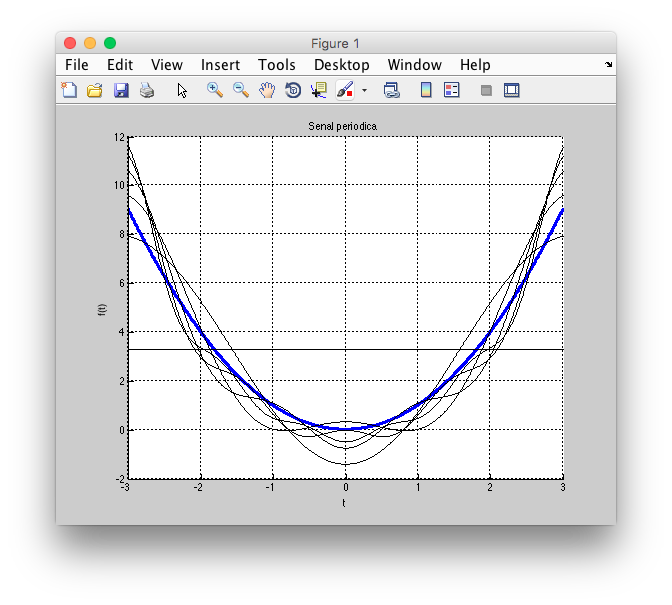
\includegraphics[width=3.5in]{imgs/sqrt.png}
\caption{Señal $f(t) = t^2$}
\label{fig_1}
\end{figure}

$\,$

\textbf{2. Desarrollar en series de Fourier}

$$f(t) = t \, sin(t),\; -\pi \leq t \leq \pi$$

\textbf{3. Desarrollar en series de Fourier}

$$f(t) = t,\; -\pi \leq t \leq \pi$$

\textbf{R/} Se plantea la serie de fourier de la siguiente manera:

$$f(t) = \frac{a_0}{2} + \sum_{n=1}^\infty\left(a_n\,cos(n\omega_0t) + b_n\,sin(n\omega_0t)\right)$$

Por lo que los coeficientes $a_x$ se pueden definir de la siguiente forma:
\begin{eqnarray*}
a_0 &=& \frac{2}{T}\int_{-T/2}^{T/2}f(t)dt\\
a_n &=& \frac{2}{T}\int_{-T/2}^{T/2}f(t)cos(n\omega_0t)dt\\
b_n &=& \frac{2}{T}\int_{-T/2}^{T/2}f(t)sin(n\omega_0t)dt
\end{eqnarray*}

Reemplazando por las variables del enunciado se llega a:
\begin{eqnarray*}
a_0 &=& \frac{1}{\pi}\int_{-\pi}^{\pi}t\,dt\\
a_n &=& \frac{1}{\pi}\int_{-\pi}^{\pi}t\,cos(n\,t)dt\\
b_n &=& \frac{1}{\pi}\int_{-\pi}^{\pi}t\,sin(n\,t)dt
\end{eqnarray*}

Resolviendo para $a_0$:
\begin{eqnarray*}
a_0 &=& \frac{1}{\pi}\int_{-\pi}^{\pi}t\,dt\\
&=& \frac{1}{\pi} \frac{t^2}{2}\bigg|_{t=-\pi}^{\pi}\\
&=& \frac{1}{2\pi} (\pi^2 - (-\pi)^2)\\
&=& 0
\end{eqnarray*}

Resolviendo para $a_n$:
\begin{eqnarray*}
a_n &=& \frac{1}{\pi}\int_{-\pi}^{\pi}t\,cos(n\,t)dt\\
&=& \frac{1}{\pi} \left(\frac{t\,sin(n\,t)}{n} + \frac{cos(n\,t)}{n^2}\right)\bigg|_{t=-\pi}^{\pi}\\
&=& \frac{\pi\,sin(n\,\pi)}{n\pi} + \frac{cos(n\,\pi)}{n^2\pi}\\
& &- \frac{(-\pi)sin(n(-\pi))}{n\pi} - \frac{cos(n(-\pi))}{n^2\pi}\\
&=& 0
\end{eqnarray*}

Resolviendo para $b_n$:
\begin{eqnarray*}
b_n &=& \frac{1}{\pi}\int_{-\pi}^{\pi}t\,sin(n\,t)dt\\
&=& \frac{1}{\pi} \left(-\frac{t\,cos(n\,t)}{n} + \frac{sin(n\,t)}{n^2}\right)\bigg|_{t=-\pi}^{\pi}\\
&=& -\frac{\pi\,cos(n\,\pi)}{n\pi} + \frac{sin(n\,\pi)}{n^2\pi}\\
& & + \frac{(-\pi)cos(n(-\pi))}{n\pi} - \frac{sin(n(-\pi))}{n^2\pi}\\
&=& \frac{2}{n}sinc(n\,\pi) -2\pi\,cosc(n\,\pi)
\end{eqnarray*}

De manera que la serie de Fourier de $f(t)$ queda de la siguiente forma:
$$f(t) = \sum_{n=1}^\infty\left(\left(\frac{2}{n}sinc(n\,\pi) -2\pi\,cosc(n\,\pi)\right)sin(n\,t)\right)$$

Esta progresión puede verse en la Figura~\ref{fig_3}, en donde a medida que se agrega un término esta sumatoria se aproxima a la señal original (mostrada en azul).

\begin{figure}[!t]
\centering
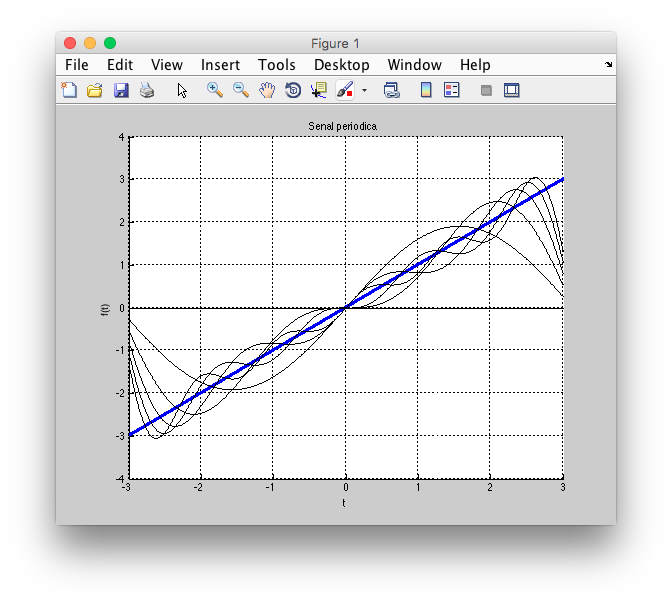
\includegraphics[width=3.5in]{imgs/lin.png}
\caption{Señal $f(t) = t$}
\label{fig_3}
\end{figure}

$\,$

\textbf{4. Desarrollar en series de Fourier}

$$f(t) = \begin{cases}
\pi +t, &-\pi \leq t \leq 0\\
t, &0 \leq t \leq \pi
\end{cases}$$

\textbf{5. Hallar el periodo}

\textbf{a)} $f(t) = sin(\frac{2\pi}{b-a}t)$

\textbf{R/} El periodo $T$ de una señal senoidal se puede definir como:

$$f(t) = sin\left(\frac{2\pi}{T}t\right)$$

Por lo que para resolver la igualdad:

$$T = (b - a)$$

Es evidente en las Figuras \ref{fig_ba4_2} y \ref{fig_ba5_2} que los periodos coinciden con los calculados.

\begin{figure}[!t]
\centering
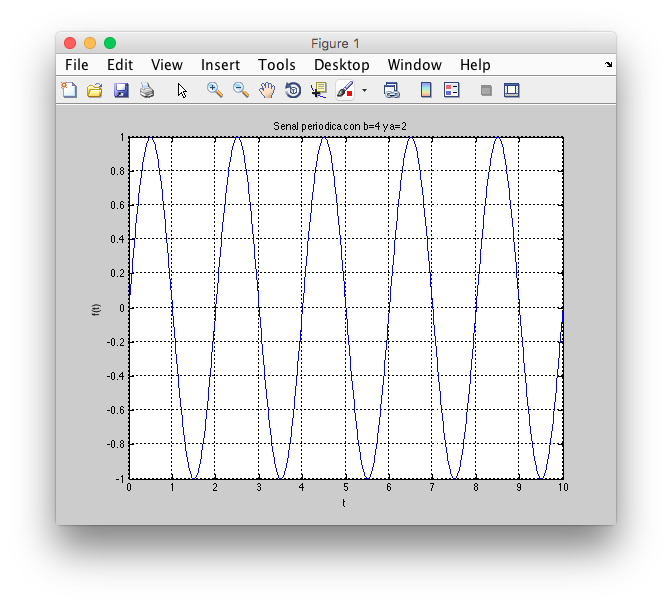
\includegraphics[width=3.5in]{imgs/ba4_2.png}
\caption{Señal $f(t) = sin(\frac{2\pi}{b-a}t)$ con $b=4$ y $a=2$}
\label{fig_ba4_2}
\end{figure}

\begin{figure}[!t]
\centering
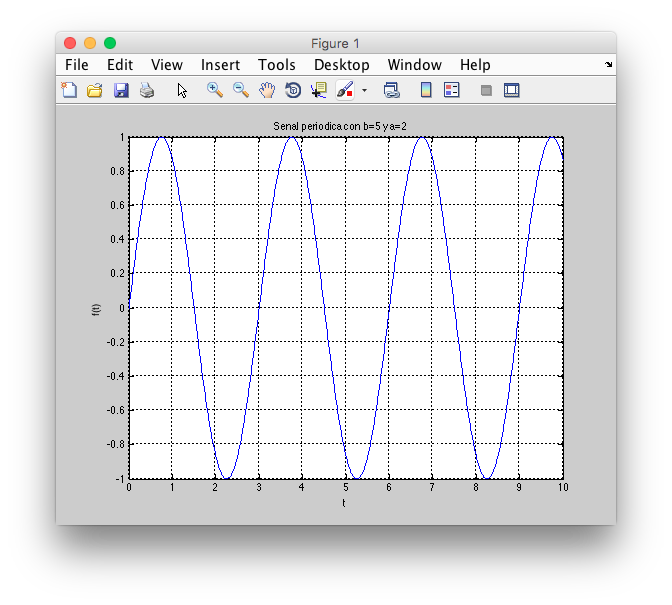
\includegraphics[width=3.5in]{imgs/ba5_2.png}
\caption{Señal $f(t) = sin(\frac{2\pi}{b-a}t)$ con $b=5$ y $a=2$}
\label{fig_ba5_2}
\end{figure}

$\,$

\textbf{b)} $f(t) = sin(t) + \frac{1}{3}sin(3t) + \frac{1}{5}sin(5t)$

\textbf{R/} El periodo $T$ de una señal senoidal se puede definir como:

$$f(t) = sin\left(\frac{2\pi}{T}t\right)$$

Por lo que para cada senoidal su periodo sería:

\begin{eqnarray*}
T_1 &=& 2\pi\\
T_2 &=& \frac{2\pi}{3}\\
T_3 &=& \frac{2\pi}{5}
\end{eqnarray*}

Dado el hecho de que la señal es una señal compuesta, será periodica si el cociente entre sus periodos es un número racional:

\begin{eqnarray*}
\frac{T_1}{T_2} &=& 3\\
\frac{T_1}{T_2} &=& 5\\
\frac{T_2}{T_3} &=& \frac{5}{3}
\end{eqnarray*}

Dado el hecho de que se cumple la condición, la señal es periódica y su periodo será en mínimo común múltiplo de estos periodos:

\begin{eqnarray*}
T &=& m.c.m(T_1,T_2,T_3)\\
&=& m.c.m(2 \pi,2\pi3^{-1},2\pi5^{-1})\\
T &=& 2\pi
\end{eqnarray*}

Es evidente en la Figura \ref{fig_5b} que el periodo coincide con el calculado.

\begin{figure}[!t]
\centering
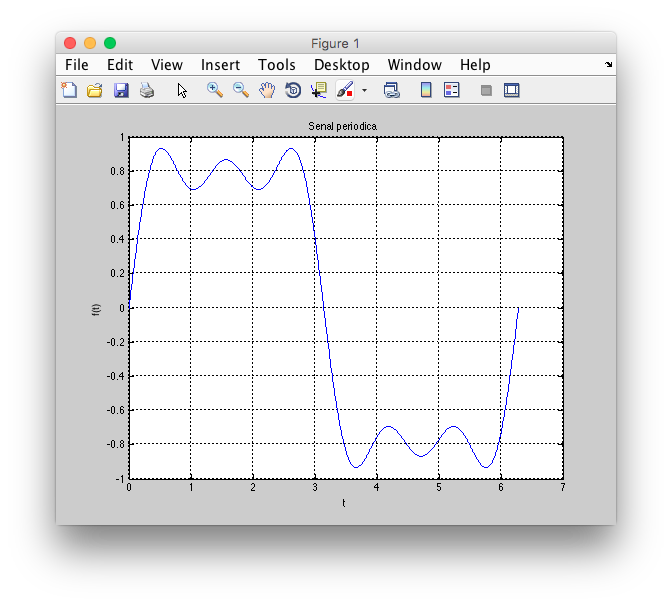
\includegraphics[width=3.5in]{imgs/5b.png}
\caption{Señal $f(t) = sin(t) + \frac{1}{3}sin(3t) + \frac{1}{5}sin(5t)$}
\label{fig_5b}
\end{figure}

$\,$

\textbf{c)} $f(t) = cos(10t) + cos((10+\pi)t)$
\end{document}
